\chapter{Blockchain Notarization: A Practical Use Case}
\label{chpr:project}
This Chapter is aimed to be a technical report of a project in which the author, in partnership with DGI (Digital Gold Institute) and ANIA (Associazione Nazionale fra le Imprese Assicuratrici), worked during the draft of this thesis.

\bigskip
\section{Executive Summary}
\label{sec:summary}
The purpose of this project work is to provide future clients a fully operating timestamping service, to enforce the notarization of digital documents which, as we already know, is traditionally achieved by certification authorities (CA), with a decentralized solution that is resilient even if the security of such CA is violated from the inside.

\bigskip
\noindent
The timestamping service is implemented, with some extensions and modification on the basis of need, according to the \textit{OpenTimestamps} protocol, because of its high scalability and low maintenance cost, all nice features that we already saw in the description of such protocol in Section \ref{sec:ots}. In addition, the proposed solution is independent of any provider, being \textit{OpenTimestamps} an open-source project. It could be made available to customers for free or in form of a subscription service, with specific service level agreements, in order to provide additional features like the custody of any user's timestamp proof, usually charged to the latter. For example, any insurance company could make use of this solution to grant authenticity of its associates' insurance policies or, more generally, whenever a digital signature is involved. We remind that \textit{OpenTimestamps} also provides all the guarantees for an independent audit: a user can verify the validity of its timestamp proof without the need of the calendar server which actually maintains the service up, just by querying a local Bitcoin node or a public block explorer. Next we will move on the technical details regarding how this service is built, specifying when the \textit{OpenTimestamps} protocol is improved.

\bigskip
\section{Architecture of the Solution}
\label{sec:architecture}
The architecture of the solution consists of three servers located in cloud, and accessible from the outside via network elements (DNS server, reverse proxy, firewall, etc.) able to transparently remap host names under the aniasafe.it domain on local IPs to the DMZ (demilitarized zone)\footnote{More precisely, a demilitarized zone is a physical or logical subnetwork that contains and exposes an organization's external-facing services to an untrusted network, usually a larger one like the Internet. All the details here: \url{https://en.wikipedia.org/wiki/DMZ_(computing)}.}.

\bigskip
\noindent
A user can easily connect to the public web server via browser at \url{https://timestamp.aniasafe.it} and upload a document to timestamp\footnote{We remind that what is really timestamped is the \textit{hash value} of such document, automatically computed on user's local device, without harming privacy. We refer to Chapter \ref{chpr:notarization} for all the details.}. It is directly from browser (thanks to the underlying JavaScript code) that the timestamp request is sent to the calendar servers to be processed. The corresponding timestamp proof is automatically downloaded on the user's local device and can be verified on the same web page, simply uploading the \colorbox{light-gray}{.ots} file. In that specific case, the browser will query public block explorers\footnote{As specified in Section \ref{sec:ots-web}, timestamping services deployed as browser applications cannot query a local Bitcoin node and have to trust public block explorers.} in order to perform the verification procedure. 

\bigskip
\noindent
Before getting into technical details regarding the code base that underlies this solution, we present two explanatory figures. On one hand, Figure \ref{fig:ots-project-stamping} is aimed to give an abstract idea of the whole timestamping process, on the other hand Figure \ref{fig:ots-project-verifying} refers to the verification procedure.

\begin{figure}[!htb]
    \centering
	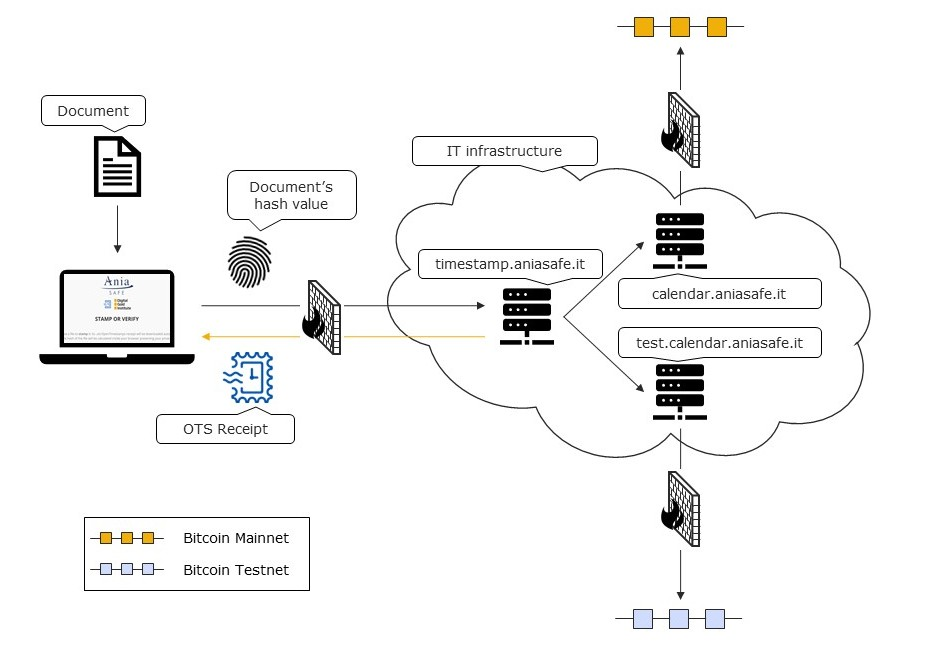
\includegraphics[width=1\linewidth]{Images/project-stamping.jpg}
	\caption{Architecture of the timestamping process}
	\label{fig:ots-project-stamping}
\end{figure}

\bigskip
\begin{figure}[!htb]
    \centering
	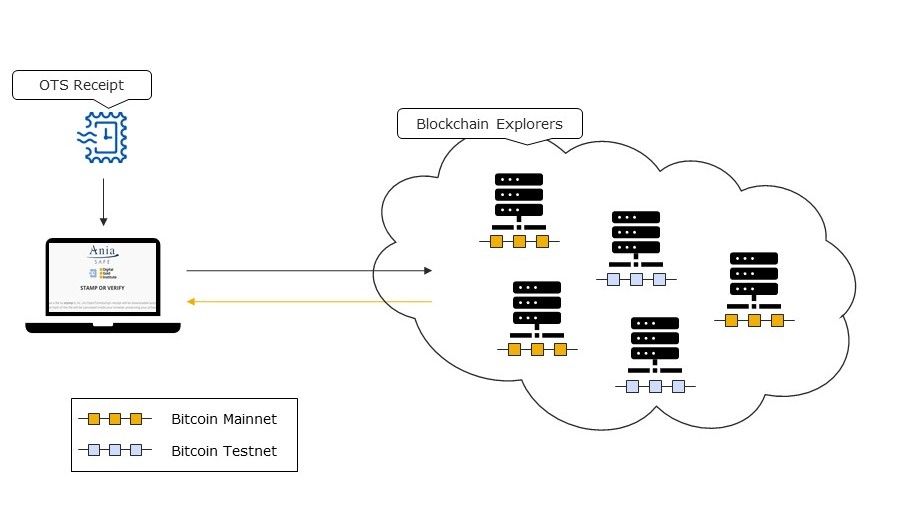
\includegraphics[width=1\linewidth]{Images/project-verifying.jpg}
	\caption{Architecture of the verification process}
	\label{fig:ots-project-verifying}
\end{figure}

\bigskip
\section{Technical Details}
The three servers introduced before are divided in a front-end server (\url{https://timestamp.aniasafe.it}) which hosts the public web page, and two back-end servers, the first one running a calendar server connected to a local\footnote{In the sense that the calendar server and the Bitcoin node run on the same machine.} Bitcoin node in mainnet mode (\url{https://calendar.aniasafe.it}), the latter connected to a local one in testnet mode (\url{https://test-calendar.aniasafe.it}).

\bigskip
\noindent
As we already know, the whole timestamping service is implemented according to the open-source \textit{OpenTimestamps} protocol. For a better understanding we will separate the client side from the server one, clarifying their functioning.

\bigskip
\subsection{Client Side}
\label{sec:client-side}
The core of the client side is the underlying JavaScript library \cite{LibraryRepositoryGitHub}, which defines the main functions invoked when a user interacts with the web interface hosted by the front-end server: \textit{stamp}, \textit{verifyTimestamp} and \textit{upgradeTimestamp}.

\begin{itemize}
    \item \textit{stamp}: it takes two parameters in input: \textit{detaches}, that is the array of detached files to stamp and \textit{options}, which specifies the calendars to send a timestamp request. First, the function makes the parsing of input parameters to check if they are in the right format. Then it invokes \textit{makeMerkleTree} that, as the name suggests, builds a merkle tree of such files and passes the root of that tree to \textit{createTimestamp}, a function that composes a timestamp and submits it to the list of calendars specified on the options parameter.
    \item \textit{verifyTimestamp}: it takes two parameters in input too: a \colorbox{light-gray}{.ots} file (the proof to be verified) and \textit{options} which, for any queried chain (f.e. Bitcoin mainnet, Bitcoin testnet, Litecoin etc.), specifies a list of block explorers and their types in order to fully manage the corresponding API\footnote{An Application Programming Interface (API) is a set of subroutine definitions, communication protocols, and tools for building software. In general terms, it is a set of clearly defined methods of communication among various components. More details here: \url{https://en.wikipedia.org/wiki/Application_programming_interface}.} in the right way. The function parses the file in input and, for any attestation found, it verifies the status of such attestation calling \textit{verifyAttestation}. If the attestation is in \textit{Pending} or \textit{Unknown} status, a warning message will notify that such attestation is incomplete or not recognized, in the sense that the tag relative to the chain used to stamp is not known. Otherwise, if the attestation is considered valid, first the function tries to reach a local node if present\footnote{We remind that verifying with a local node is always the best practice, having not to trust any third party.}, else the verification proceeds with the help of one or more block explorers. After a check of the chain in which the file is attested, it will be created an object named \textit{liteOptions} which extracts from the input parameter \textit{options} only the piece relative to the chain in question. Finally this new object is passed to the function \textit{liteVerify}\textup{\footnote{Lite or \enquote{light} because it verifies one attestaion at a time.}}, which creates an instance of the class \textit{ExplorerList}, that is a list of block explorers such function will interact to, in accordance to the ones specified in \textit{liteOptions}. These block explorers will query the blockchain with two calls, the first asking for the relative block hash, the latter, using that hash value as input, retrieves all the information of the block needed for the verification process.
    \item \textit{upgradeTimestamp}: even this function takes two parameters as input: \textit{timestamp}, that is the incomplete timestamp to upgrade and \textit{options}, which specifies the whitelisted calendars (the ones whose attestations are trusted). First it parses the input timestamp and for each attestation found it checks if it is complete or not. If incomplete, it passes a sub-timestamp (the piece of the merkle tree corresponding to a single attestation to be upgraded) and any existing completed attestation to the function \textit{UpgradeStamp}, which fills the remaining parts and merges the old attestations with the new ones.
\end{itemize}

\bigskip
\subsection{Server Side}
\label{sec:server-side}
The two back-end servers are part of the server side. They both run a calendar server connected to a local full node Bitcoin, one in mainnet mode\footnote{Mainnet is a shortcut used to indicate the main Bitcoin chain, where bitcoins have real value.}, the other in testnet mode\footnote{Like mainnet, testnet stands for the test chain, where bitcoins have no real value.}. How to run a full node Bitcoin is not of interest here, thus we remind to Appendix \ref{app:A} for a step-by-step tutorial. Instead we will focus on how to set up a calendar server, running it as a service, not just an installed program.

\bigskip
\subsection{Extensions to the protocol}
\label{sec:extensions}
A small extension to the \textit{OpenTimestamps} protocol regards the web interface. Here, the usage of the timestamp service is almost identical to the one deployed in the official web page. You can drag \& drop a document to timestamp or a \colorbox{light-gray}{.ots} file to upgrade if the timestamp is incomplete, or to verify if complete. The only modification actually visible to the eye is that the original file is no more required to start the verification process. You can check if the timestamped hash matches the original in a separate box. This allows to delegate the verification process to any third party without harming privacy, just distributing the \colorbox{light-gray}{.ots} file, which contains no information about the content of the original document. If necessary, the owner of the original document will prove the veracity of such document by showing its hash value.

\bigskip
\noindent
Obviously, this is not the end of the story. Most of the proposed extensions are not visible to the eye and they mainly relate to the underlying JavaScript library. First of all we cleaned up all the malfunctioning and inefficient (in terms of response time) block explorers invoked during the verification process, introducing Esplora, a very efficient one owned by Blockstream \cite{Blockstream}. Hence we developed a new format of the options parameter to manage the relative API correctly. More precisely we created \textit{ExplorerList}, a new father class representing a list of block explorers which, in case of need, generates an instance of one of the two child classes specifying the type: \textit{insight}, which queries the old block explorers remained in the list, and \textit{blockstream}, a new one which queries Esplora's API. A simplified example of the new options format could be:

\begin{lstlisting}
    const options = {
      bitcoin: {
        explorers: [
          {url: 'https://blockstream.info/api', type: 'blockstream'},
          {url: 'https://blockexplorer.com/api', type: 'insight'}
        ]
      },
      litecoin: {
        explorers: [
          {url: 'https://ltc-bitcore1.trezor.io/api', type: 'insight'},
          {url: 'https://insight.litecore.io/api', type: 'insight'}
        ]
      }
    }
\end{lstlisting}

\bigskip
\noindent
Another important modification of the original protocol regards the verification process and we defined it \textit{multivalidation}. 